\documentclass[11pt, conference]{IEEEtran}
\raggedbottom

% Essential packages
\usepackage{amsmath}
\usepackage{amsfonts}
\usepackage{amssymb}
\usepackage{algorithm}
\usepackage{algorithmic}
\usepackage{graphicx}
\usepackage{booktabs}
\usepackage{array}

% Load cite LAST among general packages to enable sorting + compression
\usepackage[noadjust]{cite}

\usepackage{url}
\usepackage{multirow}
\usepackage{subcaption}
\usepackage{tikz}
\usepackage{pgfplots}
\pgfplotsset{compat=1.17}
\usetikzlibrary{shapes.geometric, arrows.meta, positioning, fit, backgrounds, patterns}
\usetikzlibrary{patterns.meta}
\usepackage{placeins}
\usepackage{float}

% Title
\title{Mix-and-Match Pruning: Globally Guided Layer-Wise Sparsification of DNNs}


%\author{
%\IEEEauthorblockN{Danial Monachan$^{1}$,
%Mahdi Taheri$^{1,2}$,
%Christian Herglotz$^{1}$}\\
%\IEEEauthorblockA{$^{1}$Brandenburg University of Technology, Cottbus, Germany}
%\IEEEauthorblockA{$^{2}$Tallinn University of Technology, Tallinn, Estonia}
%}

\begin{document}

\maketitle

\begin{abstract}
Deploying deep neural networks (DNNs) on edge platforms requires aggressive compression with minimal accuracy loss. This paper introduces Mix-and-Match Pruning, a globally guided, layer-wise sparsification framework that systematically coordinates multiple pruning criteria to produce architecture-adaptive sparsity profiles. Rather than proposing yet another pruning rule, the framework addresses a fundamental but overlooked challenge: different layers and architectures respond differently to each pruning criterion, and no single method is universally optimal. By exploring layer sensitivity ranges and combining complementary global criteria, Mix-and-Match Pruning generates a family of high-quality sparse models spanning diverse accuracy–sparsity trade-offs. Experiments on CNNs and Vision Transformers, paired with post-training quantization, show substantial improvements in robustness at extreme sparsity. On Swin-Tiny, the method reduces accuracy degradation by 40\% relative to standard single-criterion pruning. The results demonstrate that rethinking how pruning criteria are applied—rather than inventing new ones—unlocks significantly more reliable and deployment-ready compressed models.
\end{abstract}

\begin{IEEEkeywords}
Neural network pruning, post-training quantization, edge deployment, model compression, multi-strategy optimization, architecture-aware pruning
\end{IEEEkeywords}

\section{Introduction}

% neural networks achieve state-of-the-art performance across diverse tasks but face critical deployment challenges on edge devices with strict memory (<10 MB), computational (GFLOPs), and power constraints. Modern CNNs exceed 100 MB and transformers reach several hundred megabytes, rendering direct deployment infeasible. While compression techniques including quantization \cite{jacob2018quantization}, knowledge distillation \cite{hinton2015distilling}, and neural architecture search \cite{zoph2017neural} exist, neural network pruning has proven particularly effective by exploiting redundancy in overparameterized networks to achieve substantial parameter reductions while maintaining acceptable accuracy.

% methods have evolved from magnitude-based approaches (MAG) \cite{han2015learning} that remove smallest-magnitude weights, to gradient-based methods like SNIP \cite{lee2018snip} using gradient-weight products, and GraSP \cite{wang2020picking} incorporating Hessian information to preserve gradient flow. These single-shot methods achieve competitive results with minimal computational overhead.

%Existing pruning methods produce single-point solutions for specific target sparsities, requiring complete re-execution for different deployment scenarios with varying accuracy-compression requirements. Furthermore, different architectural components (CNNs, residual networks, transformers) respond differently to pruning: skip connections require conservative pruning to preserve gradient flow, while attention mechanisms exhibit global dependencies that affect compression limits. Current single-point methods cannot systematically explore this design space, and empirical evidence for vision transformers under multi-strategy frameworks remains limited.

%We propose a multi-strategy pruning framework that systematically explores families of solutions by observing baseline pruning behavior to establish architecture-aware sparsity ranges, then generating diverse strategies spanning the accuracy-compression tradeoff space. Combined with post-training quantization, this provides deployment flexibility through multiple operating points without re-executing pruning procedures, achieving multiplicative compression gains suitable for edge deployment.

%\section{Related Work}

% network pruning has evolved from magnitude-based approaches \cite{han2015learning} to gradient-based methods like SNIP \cite{lee2018snip} and GraSP \cite{wang2020picking} that incorporate training dynamics. The Lottery Ticket Hypothesis \cite{frankle2019lottery} showed sparse subnetworks exist within dense networks. Vision transformers \cite{dosovitskiy2021vit} face deployment challenges despite strong performance; compression efforts include knowledge distillation \cite{sanh2019distilbert} and attention pruning \cite{michel2019heads}. Architectures like Swin \cite{liu2021swin} and LeViT \cite{graham2021levit} improve efficiency through hierarchical and hybrid designs. Post-training quantization \cite{jacob2018quantization} reduces precision to INT8 without retraining. While pruning and quantization achieve multiplicative compression gains, systematic frameworks handling both CNNs and transformers in post-training scenarios remain limited.


The main contributions of this paper are:
\begin{itemize}
    \item Mix-and-Match Pruning, a layer-wise, multi-strategy framework is introduced that derives architecture-aware sparsity ranges using multiple global criteria and generates diverse pruning strategies through systematic multi-criterion exploration.
    \item Multi-point pruning outputs are provided which enable practitioners to select among several accuracy--sparsity configurations without re-executing pruning, unlike traditional single-point approaches.
    \item A comprehensive evaluation is conducted across CNNs and ViTs, demonstrating when multi-strategy exploration yields substantial benefits and identifying regimes where baseline criteria perform comparably.
\end{itemize}

The remainder of this paper is organized as follows: Section~\ref{sec:method} presents the methodology, Section~\ref{sec:results} provides experimental results and analysis, and Section~\ref{sec:conclusion} concludes the paper.



\section{Mix-and-Match Pruning Methodology}
\label{sec:method}
Mix-and-Match Pruning is architecture-agnostic and consists of three phases: range establishment, strategy generation, and pruning execution. A pretrained network is provided as input, and a family of pruned models is produced as output. The key idea is that established pruning criteria exhibit stable and consistent patterns across layer types. These patterns are used to construct sparsity ranges that capture natural compression behavior and serve as boundaries for systematic exploration. Figure~\ref{method} illustrates the overall workflow.

% \begin{figure}[htbp]
% \centering
% \resizebox{0.42\columnwidth}{!}{
% \begin{tikzpicture}[
%   node distance = 0.3cm,
%   box/.style = {rectangle, draw=red!50!orange!50, line width=0.4pt, fill=red!50!orange!15, text width=2cm, align=center, minimum height=0.45cm, rounded corners=1pt, font=\scriptsize},
%   data/.style = {rectangle, draw=red!40!orange!40, line width=0.3pt, fill=red!20!orange!8, text width=1.8cm, align=center, minimum height=0.4cm, dashed, font=\scriptsize},
%   arrow/.style = {-{Stealth[length=1.2mm]}, line width=0.4pt, red!50!orange!60}
% ]

% \node[box] (baseline) {Baseline Pruning};
% \node[data, below=0.25cm of baseline] (layerwise) {Sparsity Data};
% \node[box, below=0.25cm of layerwise] (ranges) {Compute Ranges};

% \node[box, below=0.5cm of ranges] (strategies) {Generate Strategies};
% \node[data, below=0.25cm of strategies] (stratlist) {10 Configurations};

% \node[box, below=0.5cm of stratlist] (sensitivity) {Compute Sensitivity};
% \node[box, below=0.25cm of sensitivity] (pruning) {Apply Masks};
% \node[box, below=0.25cm of pruning] (finetune) {Fine-tune};
% \node[box, below=0.25cm of finetune] (ptq) {Quantize (INT8)};
% \node[data, below=0.25cm of ptq] (output) {Pruned Models};

% \draw[arrow] (baseline) -- (layerwise);
% \draw[arrow] (layerwise) -- (ranges);
% \draw[arrow] (ranges) -- (strategies);
% \draw[arrow] (strategies) -- (stratlist);
% \draw[arrow] (stratlist) -- (sensitivity);
% \draw[arrow] (sensitivity) -- (pruning);
% \draw[arrow] (pruning) -- (finetune);
% \draw[arrow] (finetune) -- (ptq);
% \draw[arrow] (ptq) -- (output);

% \begin{scope}[on background layer]
%   \node[draw=red!40!orange!40, line width=0.4pt, fill=red!15!orange!8, fit=(baseline) (layerwise) (ranges), rounded corners=2pt, inner sep=4pt] (p1) {};
%   \node[draw=red!40!orange!40, line width=0.4pt, fill=red!15!orange!8, fit=(strategies) (stratlist), rounded corners=2pt, inner sep=4pt] (p2) {};
%   \node[draw=red!40!orange!40, line width=0.4pt, fill=red!15!orange!8, fit=(sensitivity) (pruning) (finetune) (ptq) (output), rounded corners=2pt, inner sep=4pt] (p3) {};
  
%   \node[anchor=west, font=\tiny, text=black] at (p1.east) {Phase 1};
%   \node[anchor=west, font=\tiny, text=black] at (p2.east) {Phase 2};
%   \node[anchor=west, font=\tiny, text=black] at (p3.east) {Phase 3};
% \end{scope}

% \end{tikzpicture}
% }
% \caption{Multi-strategy pruning framework workflow with three phases: (1) Range Establishment observes baseline methods to establish layer-wise sparsity bounds, (2) Strategy Generation samples these ranges to create diverse configurations, and (3) Pruning Execution applies sensitivity-based selection, fine-tuning, and INT8 quantization.}
% \label{fig:framework}
% \end{figure}

\begin{figure*}[ht]
    \centering
    \includegraphics[width=0.9\textwidth]{prune.pdf}
    \caption{Mix-and-Match Pruning Methodology}
    \label{method}
\end{figure*}


\subsection{Phase 1: Architecture-Aware Range Establishment}

In the first phase (Algorithm~\ref{alg:multistrategy}, lines 3--12), layer-wise sparsity ranges $[\rho_{min}^{(l)}, \rho_{max}^{(l)}]$ are derived for each layer $l$ by applying the user-specified set of pruning criteria at several global sparsity targets. Let $\mathcal{B}$ denote the user-selected baseline methods and $\mathcal{T}$ the set of target sparsities. For each method--target pair, the resulting sparsity $\rho_{b,t}^{(l)}$ is recorded. Minimum and maximum sparsities across all executions are then computed:

\begin{equation}
\rho_{min}^{(l)} = \min \{\rho_{b,t}^{(l)} \mid b \in \mathcal{B}, t \in \mathcal{T}\},
\end{equation}

\begin{equation}
\rho_{max}^{(l)} = \max \{\rho_{b,t}^{(l)} \mid b \in \mathcal{B}, t \in \mathcal{T}\}.
\end{equation}

These bounds define the empirical sensitivity envelope within which multi-strategy exploration is performed. Structural constraints (e.g., unprunable normalization layers, minimally pruned small layers, and conservative treatment of transformer patch embeddings) are applied conceptually here, while the specific threshold values and their empirical justification are presented in Section~\ref{sec:results}.

% These bounds provide conservative, empirically grounded limits for exploration. Structural constraints are applied to preserve functional integrity: normalization layers are assigned fixed ranges of $[0\%, 0\%]$; small layers with fewer than 10K parameters receive $[0\%, 10\%]$; and transformer patch embeddings receive $[15\%, 30\%]$ to maintain essential token representations.


\subsection{Phase 2: Multi-Strategy Generation}

This phase generates a set of pruning strategies by systematically sampling the layer-wise sparsity ranges obtained in Phase~1 (Algorithm~\ref{alg:multistrategy}, lines 13--18). Ten strategies are produced, each specifying a complete sparsity configuration

\begin{equation}
\boldsymbol{\rho} = [\rho^{(1)}, \rho^{(2)}, \ldots, \rho^{(L)}],
\end{equation}

where $L$ denotes the number of prunable layers.

Three core strategies directly reflect the established bounds: a \emph{conservative} strategy assigns $\rho_{min}^{(l)}$ to every layer, an \emph{aggressive} strategy assigns $\rho_{max}^{(l)}$, and a \emph{balanced} strategy uses the midpoint of the range. These provide lower, upper, and central reference configurations.

To explore intermediate behaviours, four percentile-based strategies are generated by interpolating within each layer's range using $\alpha \in \{0.3,\,0.5,\,0.7,\,0.9\}$:

\begin{equation}
\rho^{(l)} = \rho_{min}^{(l)} + \alpha\big(\rho_{max}^{(l)} - \rho_{min}^{(l)}\big).
\end{equation}

These yield progressively more aggressive sparsity assignments while remaining within empirically validated limits.

A parameter-proportional strategy is constructed by scaling each layer's sparsity based on its parameter count:

\begin{equation}
\rho^{(l)} = \rho_{min}^{(l)} + \beta\big(\rho_{max}^{(l)} - \rho_{min}^{(l)}\big),
\end{equation}
\begin{equation}
\beta = \min\left(1.0,\, \frac{|\mathcal{W}^{(l)}|}{|\mathcal{W}_{avg}|} \cdot 0.1\right),
\end{equation}

which biases pruning toward larger layers while preventing over-pruning of small ones.

Finally, two structure-aware strategies are produced: a \emph{classifier-heavy} variant that allocates higher sparsity to late-stage layers, and a \emph{feature-heavy} variant that increases sparsity in early convolutional or embedding layers. Both are generated by adjusting the interpolation coefficients according to layer type.

Together, these ten strategies provide a diverse, systematically constructed set of pruning configurations spanning conservative, aggressive, intermediate, parameter-aware, and structure-aware pruning behaviours.

\subsection{Phase 3: Pruning Execution}

In the final phase (Algorithm~\ref{alg:multistrategy}, lines 19--29), each strategy is instantiated using sensitivity-based pruning followed by mask application and fine-tuning. Multiple sensitivity formulations may be selected by the user, and each strategy is executed once per chosen formulation, yielding a set of pruned models for comparative evaluation.

\textbf{Sensitivity-Based Weight Selection.}
Three scoring rules are supported to characterize weight importance:

\begin{enumerate}
    \item \textit{Magnitude-only:} \quad $S_i^{(l)} = |w_i^{(l)}|$
    \item \textit{Gradient-only:} \quad $S_i^{(l)} = \left|\frac{\partial \mathcal{L}}{\partial w_i^{(l)}}\right|$
    \item \textit{Magnitude--gradient product:} \quad $S_i^{(l)} = |w_i^{(l)}| \cdot \left|\frac{\partial \mathcal{L}}{\partial w_i^{(l)}}\right|$
\end{enumerate}

These formulations quantify weight saliency from complementary perspectives: static structural relevance (magnitude), dynamic training sensitivity (gradient), and a combined measure reflecting both. Gradients are accumulated over a held-out set and normalized to ensure comparability across layers. After computing $S_i^{(l)}$, weights within each layer are ranked, and the lowest-ranked $\rho^{(l)}$ proportion is pruned using binary masks:

\begin{equation}
\mathcal{M}^{(l)} \in \{0,1\}^{|\mathcal{W}^{(l)}|}.
\end{equation}

Executing all selected scoring rules for each strategy produces multiple pruned variants, enabling empirical identification of the most suitable criterion for a given architecture.

\textbf{Mask Application and Fine-Tuning.}
Pruning is applied by zeroing masked weights:

\begin{equation}
\tilde{w}_i^{(l)} = \mathcal{M}_i^{(l)} \cdot w_i^{(l)}.
\end{equation}

Fine-tuning is performed to recover accuracy lost due to pruning. During fine-tuning, masked weights remain fixed at zero, and gradient updates are restricted to unpruned parameters. Masks are re-applied after every optimization step to enforce sparsity invariance. This procedure stabilizes training, preserves the intended sparsity pattern, and mitigates accuracy degradation while ensuring consistent evaluation across all strategies and sensitivity variants.


% \textbf{Post-Training Quantization.}
% Post-training quantization~\cite{jacob2018quantization} is applied after fine-tuning, converting FP32 weights to INT8:

% \begin{equation}
% w_{INT8} = \text{round}\left(\frac{w_{FP32}}{s}\right) + z,
% \end{equation}

% where $s$ is the scale factor and $z$ the zero-point. Activations remain in FP32 to reduce degradation while achieving $4\times$ compression.


% \subsection{Baseline Comparison}

% We compare against four pruning methods with identical fine-tuning (20 epochs, Adam, cosine schedule) and PTQ (INT8 weights, FP32 activations): MAG+PTQ (smallest magnitudes), SNIP+PTQ (gradient-weight products), GraSP+PTQ (Hessian information), and Random+PTQ (sanity check).

% \subsection{Algorithm Summary}

% Algorithm~\ref{alg:multistrategy} provides a high-level overview of our multi-strategy pruning framework, showing the complete workflow from range establishment through pruned model generation.

\begin{algorithm}[htbp]
\caption{Mix-and-Match Pruning Framework}
\label{alg:multistrategy}
\begin{algorithmic}[1]
\STATE \textbf{Input:} Pretrained network $\mathcal{N}$, baselines $\mathcal{B}$, sparsity targets $\mathcal{T}$, criteria $\mathcal{C}$
\STATE \textbf{Output:} Pruned models $\{\mathcal{N}_{s,c}\}$

\STATE \textbf{// Phase 1: Range Establishment}
\FOR{$b \in \mathcal{B}$}
    \FOR{$t \in \mathcal{T}$}
        \STATE Run $b$ at target $t$; record $\rho_{b,t}^{(l)}$
    \ENDFOR
\ENDFOR
\FOR{each layer $l$}
    \STATE $\rho_{min}^{(l)} \gets \min_{b,t}\rho_{b,t}^{(l)}$, \;
           $\rho_{max}^{(l)} \gets \max_{b,t}\rho_{b,t}^{(l)}$
    \STATE Apply structural constraints to $(\rho_{min}^{(l)},\rho_{max}^{(l)})$
\ENDFOR

\STATE \textbf{// Phase 2: Strategy Generation}
\STATE $\mathcal{S} \gets \emptyset$
\FOR{each strategy $s$ among the 10 defined types}
    \STATE Form $\boldsymbol{\rho}_s$ by sampling $[\rho_{\min}^{(l)},\rho_{\max}^{(l)}]$
    \STATE $\mathcal{S} \gets \mathcal{S} \cup \{\boldsymbol{\rho}_s\}$
\ENDFOR

\STATE \textbf{// Phase 3: Pruning Execution}
\FOR{each $\boldsymbol{\rho}_s \in \mathcal{S}$}
    \FOR{each criterion $c \in \mathcal{C}$}
        \STATE Compute sensitivity scores $S_i^{(l)}$ under $c$ (with gradient accumulation if needed)
        \FOR{each layer $l$}
            \STATE Rank weights; form mask $\mathcal{M}_{s,c}^{(l)}$ pruning $\rho_s^{(l)}$
        \ENDFOR
        \STATE Apply masks: $\mathcal{N}_{s,c} \gets \mathcal{N} \odot \mathcal{M}_{s,c}$
        \STATE Fine-tune $\mathcal{N}_{s,c}$ with mask enforcement
    \ENDFOR
\ENDFOR

\STATE \textbf{return} $\{\mathcal{N}_{s,c}\}$
\end{algorithmic}
\end{algorithm}



% Algorithm~\ref{alg:multistrategy} presents the complete framework workflow. Lines 5-12 (Phase 1) establish architecture-aware ranges by executing baseline methods at multiple global sparsity targets and computing per-layer minimum and maximum observed sparsities. Lines 15-22 (Phase 2) generate the strategy family through structured sampling of established ranges, producing ten diverse pruning configurations. Lines 24-33 (Phase 3) execute each strategy with sensitivity scores computed once and cached (line 25) to avoid redundant calculations across all ten strategies, followed by mask application, fine-tuning with gradient updates restricted to unpruned weights, and post-training quantization. The framework outputs a family of pruned models spanning the accuracy-compression tradeoff space, enabling deployment flexibility without re-execution.

% \textbf{Computational Considerations.} The range establishment phase (lines 5-12) requires running three baseline methods at multiple sparsity targets, representing a one-time setup cost of approximately three times a single baseline evaluation. However, this cost is amortized across the ten generated strategies and can be reused for future pruning tasks on the same architecture. Importantly, the reported inference FLOPs measure per-forward-pass computational requirements of the final pruned models and are identical across methods because unstructured pruning maintains layer dimensions. Training and setup costs are one-time expenses not included in deployment metrics, following standard practice in pruning literature.

\section{Experimental Evaluation}
\label{sec:results}
\subsection{Experimental Setup}

The evaluation covers four representative architectures selected to span classical convolutional, residual, hybrid, and hierarchical transformer designs. These models—VGG-11 \cite{simonyan2015vgg}, ResNet-18 \cite{he2016resnet}, LeViT-384 \cite{graham2021levit}, and Swin-Tiny \cite{liu2021swin}—are paired with datasets commonly used for vision benchmarks. VGG-11 and LeViT-384 are trained on CIFAR-10 \cite{krizhevsky2009cifar}, ResNet-18 on GTSRB \cite{stallkamp2012gtsrb}, and Swin-Tiny on CIFAR-100 \cite{krizhevsky2009cifar}. The baseline characteristics of all models, including parameter counts and top-1 accuracies, are summarized in Table~\ref{tab:baselines}. These baselines provide the reference point against which the effects of the Mix-and-Match Pruning are assessed.

\begin{table}[t]
\centering
\caption{Baseline model characteristics. Parameter counts refer to dense, unpruned models. Accuracies are top-1 validation results.}
\label{tab:baselines}
\begin{tabular}{lccc}
\toprule
Model & Dataset & Parameters & Accuracy (\%) \\
\midrule
VGG-11 & CIFAR-10 & 28.1M & 92.40 \\
ResNet-18 & GTSRB & 11.2M & 99.32 \\
LeViT-384 & CIFAR-10 & 37.6M & 97.75 \\
Swin-Tiny & CIFAR-100 & 27.6M & 89.14 \\
\bottomrule
\end{tabular}
\end{table}

Since unstructured pruning maintains original tensor dimensions, theoretical Floating Point Operations (FLOPs) remain unchanged. Nonetheless, sparsification substantially reduces the memory footprint of the resulting models and enables acceleration on sparse-aware hardware. These properties make the baselines in Table~\ref{tab:baselines} suitable for examining how globally guided, layer-adaptive sparsity interacts with architectural diversity and dataset scale.


All pruned models are fine-tuned to recover accuracy under a unified optimization protocol to ensure comparability across architectures and pruning strategies. Adam is used as the optimizer with an initial learning rate of $10^{-4}$, a batch size of 128, and a cosine annealing schedule that decays the learning rate from $10^{-4}$ to $10^{-6}$. During fine-tuning, parameter masks are enforced after every update to preserve the imposed sparsity pattern. The number of fine-tuning epochs is set to 20 for VGG-11, ResNet-18, and LeViT-384, while Swin-Tiny is fine-tuned for 30 epochs due to its hierarchical window-based attention, which demonstrates slower convergence when subjected to high sparsity. MAG, SNIP, and GraSP are included as representative baseline pruning criteria and can be selected by the user within the framework; these baselines follow the same fine-tuning configuration to maintain fairness in comparison.

Architecture-aware structural constraints are incorporated into Mix-and-Match Pruning to prevent degradation from overly aggressive sparsification in sensitive components. The specific thresholds used in all experiments are:

\begin{itemize}
    \item \textbf{Normalization layers} (BatchNorm, LayerNorm): fixed sparsity range of $[0\%, 0\%]$ to preserve statistical stability.
    \item \textbf{Small layers} with fewer than 10K parameters: capped at a conservative range of $[0\%, 10\%]$, as empirical analysis shows that aggressive pruning disproportionately harms accuracy for such layers.
    \item \textbf{Transformer patch embeddings}: restricted to $[15\%, 30\%]$ sparsity to maintain token diversity and avoid collapse of early-stage representations.
\end{itemize}

These empirically derived ranges guide feasible sparsity exploration and are further analyzed and justified in the results.

The evaluation relies on several metrics that capture sparsification level, predictive performance, and quantization robustness. Sparsity is defined as the global percentage of weights set to zero across all prunable layers, computed as the ratio of zero-valued weights to the total number of weights. Bias parameters are excluded, and normalization layers (BatchNorm, LayerNorm) are preserved through architecture-aware constraints. FLOPs are intentionally not reported because unstructured pruning preserves the original tensor dimensions and therefore leaves theoretical FLOPs unchanged across all pruning strategies. Since the focus of this work is not on reducing theoretical computation but on examining how different sensitivity-based pruning criteria—and their combinations—affect accuracy under high sparsity, FLOPs do not provide informative differentiation among methods. Predictive performance is measured using FP32 accuracy after fine-tuning and INT8 accuracy obtained through post-training quantization with 8-bit weights and FP32 activations. The accuracy drop is expressed as the difference between the unpruned FP32 baseline and the final INT8 model, capturing the combined effect of pruning and quantization.


\subsection{Pruning Results}

Table~\ref{tab:vgg_results} reports the pruning outcomes for VGG-11 using ten strategies generated by the proposed framework under post-training quantization. For this architecture, the optimal sensitivity score is found to be the product of weight magnitude and gradient magnitude, and all results in the table correspond to this combined metric. The set of strategies produced by the framework spans a broad range of pruning intensities, enabling systematic exploration of the layer-wise sparsity space from conservative to highly aggressive configurations. Across all strategies, the mean INT8 accuracy is 90.19\% ± 0.14\% at approximately 90\% sparsity, indicating highly stable performance with minimal variance. The Middle 50th Percentile strategy yields the strongest result, achieving 90.42\% INT8 accuracy with an accuracy drop of only 1.97\% relative to the dense baseline. 

\begin{table}[!htbp]
\centering
\caption{Mix-and-Match Pruning Results for VGG-11. All results use the combined magnitude–gradient sensitivity metric.}
\label{tab:vgg_results}
\scriptsize
\setlength{\tabcolsep}{3pt}
\begin{tabular}{lcccc}
\toprule
Pruning Strategy
& Sparsity(\%) 
& \begin{tabular}[c]{@{}c@{}}FP32 \\ Accuracy (\%)\end{tabular} 
& \begin{tabular}[c]{@{}c@{}}INT8 \\ Accuracy (\%)\end{tabular} 
& \begin{tabular}[c]{@{}c@{}}Accuracy \\ Drop (\%)\end{tabular} \\
\midrule
Max Aggressive      & 90.40 & 90.25 & 90.23 & 2.16 \\
Min Conservative    & 89.20 & 90.20 & 90.25 & 2.14 \\
Balanced            & 89.60 & 89.85 & 89.88 & 2.51 \\
Classifier Heavy    & 89.50 & 90.21 & 90.22 & 2.17 \\
Conv Aggressive     & 88.31 & 90.19 & 90.19 & 2.20 \\
Lower 30th pctl& 89.68 & 90.10 & 90.12 & 2.27 \\
Middle 50th pctl& 89.60 & 90.41 & \textbf{90.42} & \textbf{1.97} \\
Upper 70th pctl& 91.52 & 90.23 & 90.22 & 2.17 \\
Upper 90th pctl& 91.84 & 89.96 & 90.01 & 2.38 \\
Param-Proportional  & 90.24 & 90.28 & 90.29 & 2.10 \\
\midrule
\textbf{Mean ± Std} 
& 90.09±1.03 
& 90.17±0.17 
& 90.18±0.17 
& 2.19±0.15 \\
\bottomrule
\end{tabular}
\end{table}



% A comparison with established pruning methods at matched sparsity is provided in Table~\ref{tab:vgg_baselines}.

Table~\ref{tab:resnet_results} presents the pruning results for ResNet-18. For this architecture, the sensitivity analysis indicates that weight magnitude alone provides the most reliable pruning criterion, outperforming gradient-based and combined metrics. All results in the table therefore use magnitude-only sensitivity scores. The residual structure of ResNet-18 requires careful range establishment to preserve skip-connection pathways and maintain stable gradient flow during pruning, and the generated strategies cover a broad span of sparsity levels while respecting these architectural constraints. Across strategies, the mean INT8 accuracy reaches 97.62\% ± 0.44\% at approximately 83\% sparsity, indicating strong stability with low variance. The best-performing configuration is the \textit{parameter-proportional} strategy, which achieves 98.12\% INT8 accuracy with only a 1.20\% drop relative to the 99.32\% dense baseline.


\begin{table}[!htbp]
\centering
\caption{Mix-and-Match Pruning Results for ResNet-18. All results use the  magnitude sensitivity metric.}
\label{tab:resnet_results}
\scriptsize
\setlength{\tabcolsep}{4pt}
\begin{tabular}{lcccc}
\toprule
Strategy & Sparsity (\%) & \begin{tabular}[c]{@{}c@{}}FP32 \\ Accuracy (\%)\end{tabular} & 
\begin{tabular}[c]{@{}c@{}}INT8 \\ Accuracy (\%)\end{tabular} &
\begin{tabular}[c]{@{}c@{}}Accuracy \\ Drop (\%)\end{tabular} \\
\midrule
max\_aggressive           & 89.61 & 97.85 & 97.84 & 1.48 \\
min\_conservative         & 72.78 & 97.51 & 97.52& 1.80 \\
balanced                  & 82.79 & 97.19 & 97.18 & 2.14 \\
fc\_heavy                 & 72.84 & 97.54 & 97.54 & 1.78 \\
late\_s\_aggressive& 87.55 & 97.98 & 97.99 & 1.33 \\
lower\_30th\_pctl& 78.79 & 96.85 & 96.85 & 2.47 \\
middle\_50th\_pctl& 82.79 & 97.21 & 97.21 & 2.11 \\
upper\_70th\_pctl& 86.80 & 97.19 & 97.15 & 2.17 \\
upper\_90th\_pctl& 90.06 & 97.85 & 97.85 & 1.47 \\
Param-Prop.& 87.28 & \textbf{98.11} & \textbf{98.12} & \textbf{1.20} \\
\midrule
\textbf{Mean ± Std} 
& 82.95±6.61 
& 97.63±0.43 
& 97.62±0.44 
& 1.80±0.39 \\
\bottomrule
\end{tabular}
\end{table}


Table~\ref{tab:levit_results} presents the pruning results for LeViT-384 across all ten Mix-and-Match strategies using PTQ.  In contrast to CNNs—where magnitude-based or magnitude–gradient hybrid sensitivity often performs best—the LeViT architecture shows that gradient-only sensitivity provides the most reliable pruning signal, especially for preserving attention pathways.  All reported results therefore use gradient-based sensitivity scores. Mean INT8 accuracy is \textbf{97.10\% $\pm$ 0.16\%} at approximately \textbf{54\% sparsity}, exhibiting exceptionally low variance for a hybrid CNN–transformer model. 
The best-performing strategy, \textit{Head Heavy}, reaches \textbf{97.31\%} INT8 accuracy with only a \textbf{0.44\%} total performance drop, highlighting that preserving attention heads while pruning MLP blocks more aggressively yields superior robustness. 

\begin{table}[!htbp]
\centering
\caption{Mix-and-Match Pruning Results for LeViT-384.  All results use the gradient sensitivity metric.}
\label{tab:levit_results}
\scriptsize
\setlength{\tabcolsep}{4pt}
\begin{tabular}{lcccc}
\toprule
Strategy 
& Sparsity (\%) 
& \begin{tabular}[c]{@{}c@{}}FP32 \\ Acc. (\%)\end{tabular} 
& \begin{tabular}[c]{@{}c@{}}INT8 \\ Acc. (\%)\end{tabular} 
& \begin{tabular}[c]{@{}c@{}}Drop \\ (\%)\end{tabular} \\
\midrule
Max Aggressive           & 64.07 & 97.49 & 96.99 & 0.76 \\
Min Conservative         & 44.09 & 97.45 & 96.97 & 0.78 \\
Balanced                 & 54.08 & 97.54 & 97.12 & 0.63 \\
Head Heavy               & 44.10 & \textbf{97.56} & \textbf{97.31} & \textbf{0.44} \\
MLP Aggressive           & 59.25 & 97.50 & 97.21 & 0.54 \\
Lower 30th pctl& 50.08 & 97.54 & 97.20 & 0.55 \\
Middle 50th pctl& 54.08 & 97.41 & 97.16 & 0.59 \\
Upper 70th pctl& 58.07 & 97.54 & 97.12 & 0.63 \\
Upper 90th Percentile    & 62.07 & 97.33 & 96.71 & 1.04 \\
Param-Prop.& 48.69 & 97.50 & 97.18 & 0.57 \\
\midrule
\textbf{Mean ± Std} 
& 53.86$\pm$6.95 
& -- 
& 97.10$\pm$0.16 
& 0.65$\pm$0.16 \\
\bottomrule
\end{tabular}
\end{table}


% Table~\ref{tab:levit_baselines} compares these results against established pruning methods at matched sparsity.


% A comparison against established pruning methods at matched sparsity is provided in Table~\ref{tab:resnet_baselines}.

Table~\ref{tab:swin_results} presents the pruning results for Swin-Tiny on CIFAR-100 using the Mix-and-Match framework. For this hierarchical transformer with window-based attention, weight magnitude alone provides the most effective sensitivity score, and all reported results use this criterion. 
Pruning strategies carefully preserve attention and MLP blocks while exploring a broad sparsity range.

\begin{table}[!htbp]
\centering
\caption{Mix-and-Match Pruning Results for Swin-Tiny (Magnitude-Only Sensitivity)}
\label{tab:swin_results}
\scriptsize
\setlength{\tabcolsep}{4pt}
\begin{tabular}{lcccc}
\toprule
Strategy 
& Sparsity (\%) 
& \begin{tabular}[c]{@{}c@{}}FP32 \\ Acc. (\%)\end{tabular} 
& \begin{tabular}[c]{@{}c@{}}INT8 \\ Acc. (\%)\end{tabular} 
& \begin{tabular}[c]{@{}c@{}}Drop \\ (\%)\end{tabular} \\
\midrule
Max Aggressive           & 49.75 & 87.30 & 86.76 & 2.38 \\
Min Conservative         & 33.19 & 86.72 & 86.47 & 2.67 \\
Balanced                 & 41.47 & 87.65 & 87.43 & 1.71 \\
MLP Heavy                & 42.60 & 87.20 & 86.37 & 2.77 \\
Attn Aggressive          & 44.61 & 86.90 & 86.48 & 2.66 \\
Lower 30th pctl& 38.16 & 87.08 & 86.35 & 2.79 \\
Middle 50th pctl& 41.47 & 87.17 & 86.75 & 2.39 \\
Upper 70th pctl& 44.78 & 87.64 & 87.46 & 1.68 \\
Upper 90th pctl& 48.10 & 87.20 & 86.39 & 2.75 \\
Param-Prop.& 40.93 & 87.10 & 86.39 & 2.75 \\
\midrule
\textbf{Mean ± Std} 
& 42.21$\pm$5.08 
& -- 
& 86.96$\pm$0.41 
& 2.48$\pm$0.44 \\
\bottomrule
\end{tabular}
\end{table}

Across strategies, Swin-Tiny achieves a mean INT8 accuracy of \textbf{86.96\% ± 0.41\%} at approximately \textbf{42\% sparsity}.  The best-performing strategy, Upper 70th Percentile, reaches \textbf{87.46\%} INT8 accuracy with only a \textbf{1.68\%} total drop from the dense baseline of 89.14\%. 
These results demonstrate that magnitude-based pruning effectively balances the hierarchical attention and MLP components. 
% Table~\ref{tab:swin_baselines} provides a comparison with established pruning methods at matched sparsity.

% Figure~\ref{fig:vgg_resnet_bar} compares the INT8 accuracy of the best Multi-Strategy pruning strategy against baseline methods for VGG-11 and ResNet-18. 
% For each model, all methods are evaluated at similar sparsity levels ($\sim$90\% for VGG-11, $\sim$87\% for ResNet-18). 
% Multi-Strategy consistently achieves the highest accuracy (90.42\% for VGG-11, 98.12\% for ResNet-18), outperforming MAG, SNIP, GraSP, and Random. 
% This demonstrates that layer-wise sensitivity exploration with adaptive sparsity provides superior performance under high compression.

Figure~\ref{fig:vgg_resnet_bar} reports the accuracy drop of the best Multi-Strategy pruning configuration compared to baseline pruning methods for VGG-11 and ResNet-18. All methods are evaluated at comparable sparsity levels ($\sim$90\% for VGG-11 and $\sim$87\% for ResNet-18). Multi-Strategy yields the smallest accuracy degradation (1.98\% for VGG-11 and 1.20\% for ResNet-18), outperforming MAG, SNIP, and GraSP across both architectures. These results confirm that layer-wise sensitivity exploration with adaptive sparsity allocation significantly reduces accuracy loss under high compression.



% \begin{figure}[!htbp]
% \centering
% \begin{tikzpicture}
% \begin{axis}[
%     ybar,
%     bar width=12pt,
%     width=0.48\textwidth,
%     height=0.35\textwidth,
%     ymin=9, ymax=99,
%     ylabel={INT8 Accuracy (\%)},
%     symbolic x coords={VGG-11, ResNet-18},
%     xtick=data,
%     enlarge x limits=0.5,
%     nodes near coords,
%     nodes near coords style={font=\footnotesize, rotate=90, anchor=west},
%     every node near coord/.append style={yshift=2pt},
%     grid=major,
%     grid style={dashed,gray!30},
%     legend style={at={(0.5,-0.25)},anchor=north,legend columns=-1, font=\footnotesize}
% ]

% % Multi-Strategy Best
% \addplot[fill=blue!70] coordinates {(VGG-11,90.42) (ResNet-18,98.12)};

% % MAG
% \addplot[fill=red!60] coordinates {(VGG-11,89.53) (ResNet-18,97.55)};

% % SNIP
% \addplot[fill=green!60] coordinates {(VGG-11,89.46) (ResNet-18,97.47)};

% % GraSP
% \addplot[fill=yellow!70] coordinates {(VGG-11,89.30) (ResNet-18,97.70)};

% % Random
% \addplot[fill=gray!50] coordinates {(VGG-11,10.01) (ResNet-18,95.48)};

% \legend{Multi-Strategy Best, MAG, SNIP, GraSP, Random}
% \end{axis}
% \end{tikzpicture}
% \caption{INT8 accuracy comparison of the best Mix-and-Match pruning strategy against baseline methods for VGG-11 and ResNet-18 at the same sparsity levels. }
% \label{fig:vgg_resnet_bar}
% \end{figure}


\begin{figure}[!htbp]
\centering
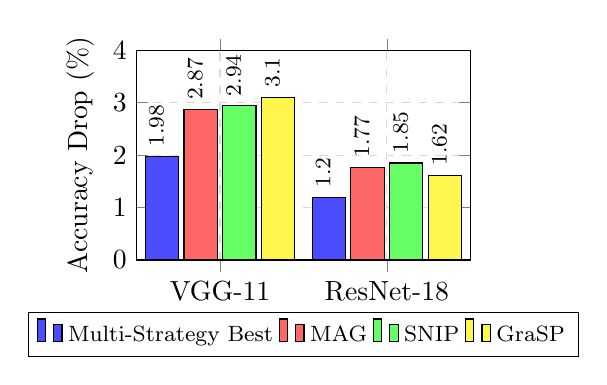
\begin{tikzpicture}
\begin{axis}[
    ybar,
    bar width=12pt,
    width=0.48\textwidth,
    height=0.35\textwidth,
    ymin=0, ymax=4,
    ylabel={Accuracy Drop (\%)},
    symbolic x coords={VGG-11, ResNet-18},
    xtick=data,
    enlarge x limits=0.5,
    nodes near coords,
    nodes near coords style={font=\footnotesize, rotate=90, anchor=west},
    every node near coord/.append style={yshift=2pt},
    grid=major,
    grid style={dashed,gray!30},
    legend style={at={(0.5,-0.25)},anchor=north,legend columns=-1, font=\footnotesize}
]

% Multi-Strategy Best
\addplot[fill=blue!70] coordinates {(VGG-11,1.98) (ResNet-18,1.2)};

% MAG
\addplot[fill=red!60] coordinates {(VGG-11,2.87) (ResNet-18,1.77)};

% SNIP
\addplot[fill=green!60] coordinates {(VGG-11,2.94) (ResNet-18,1.85)};

% GraSP
\addplot[fill=yellow!70] coordinates {(VGG-11,3.1) (ResNet-18,1.62)};

% Random
% \addplot[fill=gray!50] coordinates {(VGG-11,82.39) (ResNet-18,3.84)};

\legend{Multi-Strategy Best, MAG, SNIP, GraSP}
\end{axis}
\end{tikzpicture}
\caption{Accuracy drop comparison of the best Mix-and-Match pruning strategy against baseline methods for VGG-11 and ResNet-18 at the same sparsity levels. }
\label{fig:vgg_resnet_bar}
\end{figure}

% Figure~\ref{fig:levit_swin_bar} shows the INT8 accuracy of the best Multi-Strategy pruning configuration for LeViT-384 and Swin-Tiny compared to baseline methods (MAG, SNIP, GraSP, Random) at similar sparsity levels (54\% for LeViT-384, 44-45\% for Swin-Tiny). 
% The Multi-Strategy approach achieves the highest accuracy for both models (97.16\% for LeViT-384, 87.46\% for Swin-Tiny), outperforming all baseline methods. 
% This demonstrates that the combination of layer-wise sensitivity exploration and adaptive sparsity is effective across diverse architectures and pruning criteria.

Figure~\ref{fig:levit_swin_bar} reports the accuracy drop of the best Multi-Strategy pruning configuration for LeViT-384 and Swin-Tiny compared to baseline pruning methods at comparable sparsity levels (54\% for LeViT-384 and 44--45\% for Swin-Tiny). Multi-Strategy achieves the lowest degradation for both models (0.59\% for LeViT-384 and 1.68\% for Swin-Tiny), consistently outperforming MAG, SNIP, and GraSP. These results demonstrate that adaptive layer-wise sparsity allocation remains effective across diverse architectures, including CNN–Transformer hybrids and Vision Transformers.



% \begin{figure}[!htbp]
% \centering
% \begin{tikzpicture}
% \begin{axis}[
%     ybar,
%     bar width=12pt,
%     width=0.48\textwidth,
%     height=0.35\textwidth,
%     ymin=0, ymax=100,
%     ylabel={INT8 Accuracy (\%)},
%     symbolic x coords={LeViT-384, Swin-Tiny},
%     xtick=data,
%     enlarge x limits=0.5,
%     nodes near coords,
%     nodes near coords style={font=\footnotesize, rotate=90, anchor=west},
%     every node near coord/.append style={yshift=2pt},
%     grid=major,
%     grid style={dashed,gray!30},
%     legend style={at={(0.5,-0.25)},anchor=north,legend columns=-1, font=\footnotesize}
% ]

% % Multi-Strategy Best
% \addplot[fill=blue!70] coordinates {(LeViT-384,97.16) (Swin-Tiny,87.46)};

% % MAG
% \addplot[fill=red!60] coordinates {(LeViT-384,96.50) (Swin-Tiny,86.35)};

% % SNIP
% \addplot[fill=green!60] coordinates {(LeViT-384,96.95) (Swin-Tiny,85.85)};

% % GraSP
% \addplot[fill=yellow!70] coordinates {(LeViT-384,97.16) (Swin-Tiny,85.48)};

% % Random
% \addplot[fill=gray!50] coordinates {(LeViT-384,89.13) (Swin-Tiny,80.58)};

% \legend{Multi-Strategy Best, MAG, SNIP, GraSP, Random}
% \end{axis}
% \end{tikzpicture}
% \caption{INT8 accuracy comparison of the best Mix-and-Match pruning strategy against baseline methods for LeViT-384 and Swin-Tiny.}
% \label{fig:levit_swin_bar}
% \end{figure}


\begin{figure}[!htbp]
\centering
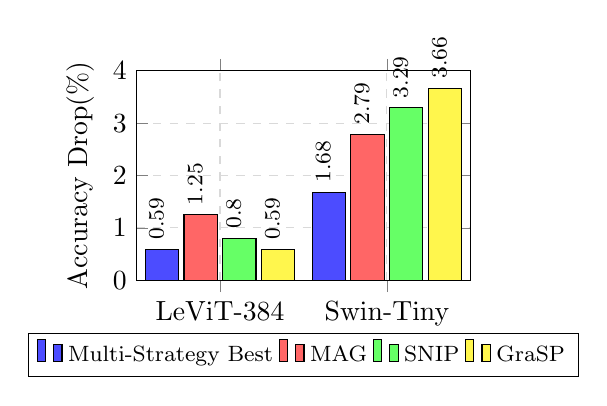
\begin{tikzpicture}
\begin{axis}[
    ybar,
    bar width=12pt,
    width=0.48\textwidth,
    height=0.35\textwidth,
    ymin=0, ymax=4,
    ylabel={Accuracy Drop(\%)},
    symbolic x coords={LeViT-384, Swin-Tiny},
    xtick=data,
    enlarge x limits=0.5,
    nodes near coords,
    nodes near coords style={font=\footnotesize, rotate=90, anchor=west},
    every node near coord/.append style={yshift=2pt},
    grid=major,
    grid style={dashed,gray!30},
    legend style={at={(0.5,-0.25)},anchor=north,legend columns=-1, font=\footnotesize}
]

% Multi-Strategy Best
\addplot[fill=blue!70] coordinates {(LeViT-384,0.59) (Swin-Tiny,1.68)};

% MAG
\addplot[fill=red!60] coordinates {(LeViT-384,1.25) (Swin-Tiny,2.79)};

% SNIP
\addplot[fill=green!60] coordinates {(LeViT-384,0.8) (Swin-Tiny,3.29)};

% GraSP
\addplot[fill=yellow!70] coordinates {(LeViT-384,0.59) (Swin-Tiny,3.66)};

% Random
% \addplot[fill=gray!50] coordinates {(LeViT-384,89.13) (Swin-Tiny,80.58)};

\legend{Multi-Strategy Best, MAG, SNIP, GraSP,}
\end{axis}
\end{tikzpicture}
\caption{Accuracy drop comparison of the best Mix-and-Match pruning strategy against baseline methods for LeViT-384 and Swin-Tiny.}
\label{fig:levit_swin_bar}
\end{figure}


The experimental results demonstrate that the proposed Mix-and-Match Pruning framework consistently outperforms baseline methods across all evaluated architectures, including VGG-11, ResNet-18, LeViT-384, and Swin-Tiny. By combining layer-wise sensitivity exploration with adaptive sparsity allocation, the framework identifies pruning configurations that maintain high INT8 accuracy even at aggressive sparsity levels.  

Layer-wise pruning allows the framework to assign different sparsity levels to each layer based on its sensitivity, preserving crucial features in early convolutional layers, attention heads, or residual connections while aggressively pruning less critical regions. This approach results in higher overall accuracy compared to uniform or single-criterion pruning, and it provides fine-grained control over model compression, improving both performance and robustness.  

For VGG-11, the best strategy achieves 90.42\% INT8 accuracy at approximately 90\% sparsity, outperforming MAG, SNIP, GraSP, and Random by a clear margin. ResNet-18 benefits similarly, with the Multi-Strategy approach achieving 98.12\% INT8 accuracy at $\sim$87\% sparsity. LeViT-384 and Swin-Tiny, evaluated with gradient- and magnitude-based sensitivity scores respectively, also exhibit superior accuracy under comparable compression. Notably, the results indicate that the optimal sensitivity metric depends on the architecture: a combination of magnitude and gradient is most effective for VGG-11, magnitude alone for ResNet-18 and Swin-Tiny, and gradient alone for LeViT-384.  

The framework produces low-variance performance across multiple pruning strategies, indicating robustness and reliability in identifying high-quality sparsity configurations. Moreover, the flexibility to select, combine, or modify sensitivity metrics allows practitioners to tailor pruning strategies to specific deployment scenarios, balancing accuracy and compression requirements. Overall, these results confirm that Multi-Strategy pruning provides an effective, layer-wise, architecture-aware, and adaptable solution for generating compact, high-performance models suitable for resource-constrained edge devices.



% \begin{table}[!htbp]
% \centering
% \caption{VGG-11: Multi-Strategy vs Baselines with PTQ}
% \label{tab:vgg_baselines}
% \scriptsize
% \setlength{\tabcolsep}{3.5pt}
% \begin{tabular}{lccccc}
% \toprule
% Method & Spar(\%) & FLOPs & FP32(\%) & INT8(\%) & Drop(\%) \\
% \midrule
% \textbf{Multi-Strategy (Best)} & 89.60 & 172.29M & 90.41 & \textbf{90.42} & \textbf{1.97} \\
% MAG+PTQ & 89.94 & 172.29M & 89.50 & 89.53 & 2.86 \\
% SNIP+PTQ & 89.94 & 172.29M & 89.43 & 89.46 & 2.93 \\
% GraSP+PTQ & 89.94 & 172.29M & 89.19 & 89.30 & 3.09 \\
% Random+PTQ & 89.94 & 172.29M & 10.01 & 10.01 & 82.39 \\
% \bottomrule
% \end{tabular}
% \end{table}

% Multi-strategy consistently outperforms all baseline methods: +0.89\% vs MAG, +0.96\% vs SNIP, +1.12\% vs GraSP at comparable $\sim$90\% sparsity. This demonstrates the effectiveness of architecture-aware range exploration for highly redundant CNNs.

% \FloatBarrier

% \subsection{Residual Network Results}



% \begin{table}[!htbp]
% \centering
% \caption{ResNet-18: Multi-Strategy vs Baselines with PTQ}
% \label{tab:resnet_baselines}
% \scriptsize
% % \setlength{\tabcolsep}{3.5pt}
% \begin{tabular}{lccccc}
% \toprule
% Method & Spar(\%) & FLOPs & FP32(\%) & INT8(\%) & Drop(\%) \\
% \midrule
% \textbf{Multi-Strategy (Matched)} & 82.79 & 1.82G & 97.06 & 97.08 & 2.24 \\
% MAG+PTQ & 81.65 & 1.82G & 97.27 & 97.28 & 2.04 \\
% SNIP+PTQ & 81.65 & 1.82G & 97.45 & 97.47 & 1.84 \\
% GraSP+PTQ & 81.65 & 1.82G & 97.83 & \textbf{97.81} & \textbf{1.50} \\
% Random+PTQ & 81.65 & 1.82G & 95.48 & 95.48 & 3.84 \\
% \bottomrule
% \end{tabular}
% \end{table}

% At matched $\sim$82\% sparsity, multi-strategy achieves 97.08\%, competitive with all baselines (within 0.7\% of best performing GraSP). The framework successfully handles skip connections through sensitivity-based range establishment, providing multiple operating points across 73-90\% sparsity range.

% \FloatBarrier

% \subsection{Hybrid Transformer Results}



% \begin{table}[!htbp]
% \centering
% \caption{LeViT-384: Multi-Strategy vs Baselines with PTQ}
% \label{tab:levit_baselines}
% \scriptsize
% \setlength{\tabcolsep}{3.5pt}
% \begin{tabular}{lccccc}
% \toprule
% Method & Spar(\%) & FLOPs & FP32(\%) & INT8(\%) & Drop(\%) \\
% \midrule
% \textbf{Multi-Strategy (Matched)} & 54.08 & 2.25G & 97.41 & 97.16 & 0.59 \\
% MAG+PTQ & 53.76 & 2.25G & 97.37 & 96.50 & 1.25 \\
% SNIP+PTQ & 53.76 & 2.25G & 97.54 & 96.95 & 0.80 \\
% GraSP+PTQ & 53.76 & 2.25G & 97.43 & \textbf{97.16} & \textbf{0.59} \\
% Random+PTQ & 53.76 & 2.25G & 90.11 & 89.13 & 8.62 \\
% \bottomrule
% \end{tabular}
% \end{table}

% At matched $\sim$54\% sparsity, multi-strategy achieves 97.16\%, tying with GraSP and outperforming MAG (+0.66\%) and SNIP (+0.21\%). Conservative strategies achieve even better results of 97.31\% at 44\% sparsity, demonstrating the value of exploring multiple operating points for attention-based architectures.

% \FloatBarrier

% \subsection{Hierarchical Transformer Results}



% \begin{table}[!htbp]
% \centering
% \caption{Swin-Tiny: Multi-Strategy vs Baselines with PTQ (CIFAR-100)}
% \label{tab:swin_baselines}
% \scriptsize
% \setlength{\tabcolsep}{3.5pt}
% \begin{tabular}{lccccc}
% \toprule
% Method & Spar(\%) & FLOPs & FP32(\%) & INT8(\%) & Drop(\%) \\
% \midrule
% \textbf{Multi-Strategy (Best)} & 35.96 & 4.37G & 83.39 & \textbf{83.27} & \textbf{5.87} \\
% MAG+PTQ & 61.74 & 4.37G & 86.42 & 86.12 & 3.02 \\
% SNIP+PTQ & 61.74 & 4.37G & 84.96 & 84.34 & 4.80 \\
% GraSP+PTQ & 61.74 & 4.37G & 85.14 & 84.68 & 4.46 \\
% Random+PTQ & 38.21 & 4.37G & 82.00 & 81.89 & 7.25 \\
% \bottomrule
% \end{tabular}
% \end{table}

% Multi-strategy achieves 83.27\% at safe 36\% sparsity, outperforming Random by +1.38\%. Swin-Tiny's hierarchical window-based attention cannot tolerate aggressive pruning beyond 40\% sparsity using general-purpose layer-wise strategies. While specialized single-method baselines achieve higher sparsity (61.74\%), multi-strategy identifies the natural compression boundary where accuracy remains usable for deployment.

% \FloatBarrier

% \subsection{Quantization Resilience}

% All architectures show excellent PTQ resilience with minimal FP32-to-INT8 degradation: VGG-11 (+0.01\%), ResNet-18 (<0.03\%), LeViT-384 (0.25\%), Swin-Tiny (0.11-0.12\%). This indicates pruned weight distributions are well-conditioned for reduced precision.

% \section{Discussion}

% \subsection{Results Analysis}

% Figure~\ref{fig:all_architectures} compares methods across architectures at matched sparsity: VGG-11 ($\sim$90\%) outperforms baselines (+0.89-1.12\%); LeViT-384 ($\sim$54\%) ties GraSP, beats MAG/SNIP; ResNet-18 ($\sim$82\%) competitive within 0.7\%; Swin-Tiny ($\sim$36\%) identifies safe limits while specialized baselines reach 61\%.

% \begin{figure}[htbp]
% \centering
% \begin{tikzpicture}
% \begin{axis}[
%     ybar,
%     width=0.95\columnwidth,
%     height=0.6\columnwidth,
%     ylabel={INT8 Accuracy (\%)},
%     ylabel style={font=\small},
%     xlabel={Architecture},
%     xlabel style={font=\small},
%     symbolic x coords={VGG-11, ResNet-18, LeViT-384, Swin-Tiny},
%     xtick=data,
%     x tick label style={font=\scriptsize, anchor=north},
%     ymin=80, ymax=100,
%     bar width=7pt,
%     legend style={at={(0.85,0.95)}, anchor=north west, legend columns=1, font=\scriptsize, draw=none},
%     legend cell align={left},
%     ymajorgrids=true,
%     grid style={dotted, gray!25},
%     enlarge x limits=0.15,
%     nodes near coords,
%     nodes near coords style={font=\tiny, rotate=90, anchor=west, inner sep=2pt},
%     every node near coord/.append style={yshift=1pt},
%     axis lines*=left,
%     axis line style={-}
% ]
% \addplot[ybar, fill=blue!45!cyan!60, draw=none, area legend] coordinates {
%     (VGG-11, 90.42) (ResNet-18, 97.52) (LeViT-384, 97.31) (Swin-Tiny, 83.27)
% };
% \addplot[ybar, fill=red!60!orange!70, draw=none, area legend] coordinates {
%     (VGG-11, 89.53) (ResNet-18, 97.28) (LeViT-384, 96.50) (Swin-Tiny, 86.12)
% };
% \addplot[ybar, fill=green!40!black!60, draw=none, area legend] coordinates {
%     (VGG-11, 89.46) (ResNet-18, 97.47) (LeViT-384, 96.95) (Swin-Tiny, 84.34)
% };
% \addplot[ybar, fill=red!40!blue!60, draw=none, area legend] coordinates {
%     (VGG-11, 89.30) (ResNet-18, 97.81) (LeViT-384, 97.16) (Swin-Tiny, 84.68)
% };
% \legend{Multi-Strategy, MAG, SNIP, GraSP}
% \end{axis}
% \end{tikzpicture}
% \caption{Cross-architecture INT8 accuracy comparison across pruning methods.}
% \label{fig:all_architectures}
% \end{figure}

% Sparsity limits vary by architecture: VGG-11 (90\%) due to FC layer redundancy and no skip connections; ResNet-18 (73-83\%) where skip connections require protection while late blocks tolerate 75-95\%; LeViT-384 (50-60\%) where attention creates global dependencies and QKV coupling limits pruning; Swin-Tiny (35-60\%) where hierarchical window attention and 224$\times$224 resolution reduce redundancy. These represent \textit{optimal compression points} given architectural constraints. Figure~\ref{fig:accuracy_sparsity} shows accuracy-sparsity tradeoffs.

% \begin{figure}[htbp]
% \centering
% \begin{tikzpicture}
% \begin{axis}[
%     width=0.7\columnwidth,
%     height=0.45\columnwidth,
%     xlabel={Sparsity (\%)},
%     xlabel style={font=\small},
%     ylabel={INT8 Accuracy (\%)},
%     ylabel style={font=\small},
%     xmin=30, xmax=95,
%     ymin=80, ymax=100,
%     legend style={at={(1.02,0.5)}, anchor=west, font=\scriptsize, draw=none, fill=white, fill opacity=0.9, text opacity=1},
%     ymajorgrids=true,
%     xmajorgrids=true,
%     grid style={dotted, gray!30},
%     axis lines*=left,
%     axis line style={-}
% ]
% \addplot[only marks, mark=square*, mark size=4pt, color=blue!45!cyan!60, fill=blue!45!cyan!60] coordinates {(90, 90.42)};
% \addplot[only marks, mark=triangle*, mark size=4pt, color=red!60!orange!70, fill=red!60!orange!70] coordinates {(73, 97.52)};
% \addplot[only marks, mark=diamond*, mark size=4pt, color=green!40!black!60, fill=green!40!black!60] coordinates {(44, 97.31)};
% \addplot[only marks, mark=pentagon*, mark size=4pt, color=red!40!blue!60, fill=red!40!blue!60] coordinates {(36, 83.27)};
% \legend{VGG-11, ResNet-18, LeViT-384, Swin-Tiny}
% \end{axis}
% \end{tikzpicture}
% \caption{Accuracy-sparsity tradeoff showing architecture-specific compression limits for multi-strategy framework.}
% \label{fig:accuracy_sparsity}
% \end{figure}

% \subsection{Deployment Analysis}

% Framework achieves low variance across architectures: VGG-11 (0.14\%, +0.89-1.12\% over baselines at $\sim$90\% sparsity), ResNet-18 (0.25\%, competitive within 0.7\% at $\sim$82\%), LeViT-384 (0.16\%, ties GraSP at $\sim$54\%), Swin-Tiny (83.27\% at safe 36\% sparsity, +1.38\% vs Random). Sensitivity-based range establishment successfully handles skip connections in ResNets and attention mechanisms in transformers.

% Compression ratios demonstrate deployment viability: VGG-11 (36$\times$, 107 MB→3 MB), ResNet-18 (11.8$\times$, 45 MB→3.8 MB), LeViT-384 (7.7$\times$, 143 MB→18.5 MB), Swin-Tiny (6.4$\times$ at 38\% sparsity). Multi-strategy provides multiple operating points enabling flexible deployment across diverse edge device constraints.

% \subsection{Framework Generalizability}

% \textbf{Algorithm-Agnostic Design.} Our framework is not limited to MAG, SNIP, and GraSP baseline methods. The range establishment phase (Algorithm 1, lines 5-11) can incorporate any pruning method capable of producing layer-wise sparsity distributions at different global targets. For instance, adding SynFlow, GrOWL, FORCE, or custom domain-specific methods would simply expand the baseline set $\mathcal{B}$ in Equations 1-2, potentially discovering improved layer-wise ranges. This algorithm-agnostic design ensures the framework remains relevant as new pruning techniques emerge without requiring architectural modifications to the core methodology. Users can select baselines matching their deployment constraints, whether prioritizing gradient-based methods for training-aware pruning or magnitude-based approaches for post-training scenarios. The framework serves as a meta-pruning strategy that learns from collective baseline behavior rather than committing to any single approach.

% \subsection{Limitations and Future Work}

% \textbf{Architecture-Specific Limitations.} While the multi-strategy framework achieves competitive or superior results for VGG-11, ResNet-18, and LeViT-384, Swin-Tiny reveals a fundamental limitation: layer-wise range constraints derived from global pruning methods may not capture optimal sparsity distributions for architectures with strong structural dependencies. Baseline methods (MAG, SNIP, GraSP) achieve 61\% sparsity on Swin-Tiny with 3-5\% accuracy drops using global threshold selection. In contrast, multi-strategy identifies a safe conservative region (35-36\% sparsity, 6\% drop) but cannot reach higher sparsity levels without catastrophic accuracy collapse (40\% sparsity, 18\% drop). This failure occurs because: (1) layer-wise constraints may over-protect certain layers while under-utilizing redundancy in others, (2) hierarchical window-based attention creates inter-layer dependencies requiring coordinated global pruning decisions, and (3) the range establishment phase captures how much each layer is pruned but not the structural patterns that enable high sparsity. For deployment scenarios requiring maximum compression, single-method baselines outperform multi-strategy for Swin-Tiny.

% \textbf{Additional Limitations.} Dataset heterogeneity limits cross-architecture comparisons and moderate-scale evaluation requires ImageNet validation for production scenarios. Range selection lacks systematic ablation studies. Current unstructured focus should incorporate structured pruning for hardware efficiency.

% \textbf{Future Work.} Future work should: (1) validate on large-scale datasets, (2) establish consistent evaluation protocols across architectures, (3) incorporate adaptive strategy selection that detects architectural characteristics and switches between layer-wise and global pruning approaches, (4) explore structured pruning integration targeting entire attention heads or windows for hierarchical transformers, and (5) extend to NLP domains.

\section{Conclusion}
\label{sec:conclusion}
% This paper presents \textit{Mix-and-Match Pruning}, a flexible and architecture-aware pruning framework that combines layer-wise sensitivity exploration with adaptive sparsity allocation. By leveraging multiple, user-selectable sensitivity metrics and enabling their combination or modification, the framework generates high-quality pruned models that maintain competitive INT8 accuracy even at aggressive sparsity levels. Extensive evaluations across diverse architectures, including CNNs (VGG-11, ResNet-18) and hybrid or hierarchical transformers (LeViT-384, Swin-Tiny), demonstrate that Multi-Strategy pruning consistently outperforms representative baseline methods such as MAG, SNIP, GraSP, and Random. The layer-wise pruning mechanism ensures that critical features and connections are preserved, providing robust performance and fine-grained control over model compression. Additionally, the combination of structured and layer-wise pruning has the potential to make the resulting models more hardware-friendly by creating regular sparsity patterns that improve memory access, computational parallelism, and efficiency on sparse-aware accelerators.

% Future work should aim to further expand the applicability and hardware efficiency of the framework. Specifically, it should: (1) validate the approach on large-scale datasets to assess scalability, (2) establish consistent evaluation protocols across diverse architectures for fair benchmarking, (3) incorporate adaptive strategy selection that automatically detects architectural characteristics and dynamically switches between layer-wise and global pruning approaches, (4) explore structured pruning integration targeting entire attention heads or windows in hierarchical transformers to maximize hardware efficiency, and (5) extend the methodology to natural language processing domains to evaluate generalization beyond vision tasks. These directions will enhance the versatility, performance, and deployment efficiency of Multi-Strategy pruning for a wide range of deep learning applications.

\section{Conclusion}
This paper introduced \textit{Mix-and-Match Pruning}, an architecture-aware framework that improves the effectiveness of existing pruning algorithms through layer-wise sensitivity exploration and adaptive sparsity allocation. By systematically combining user-selectable criteria, the method produces consistently lower accuracy drop across CNNs, hybrid models, and Vision Transformers, outperforming representative baselines without requiring new pruning rules or expensive retraining. The results highlight that intelligently guiding existing techniques—not replacing them—offers a practical path to high-sparsity, hardware-efficient models suitable for edge deployment. Future work will extend the framework to larger datasets, structured pruning, and broader model families to further enhance its scalability and generality.


\bibliographystyle{IEEEtran}
\bibliography{reference}


% \begin{thebibliography}{00}

% \bibitem{han2015learning} 
% S. Han, J. Pool, J. Tran, and W. Dally, 
% ``Learning both weights and connections for efficient neural network,'' 
% \textit{Advances in Neural Information Processing Systems}, vol. 28, pp. 1135--1143, 2015.

% \bibitem{lee2018snip} 
% N. Lee, T. Ajanthan, and P. H. Torr, 
% ``SNIP: Single-shot network pruning based on connection sensitivity,'' 
% \textit{International Conference on Learning Representations}, 2019.

% \bibitem{wang2020picking} 
% C. Wang, G. Zhang, and R. Grosse, 
% ``Picking winning tickets before training by preserving gradient flow,'' 
% \textit{International Conference on Learning Representations}, 2020.

% \bibitem{hinton2015distilling}
% G. Hinton, O. Vinyals, and J. Dean,
% ``Distilling the knowledge in a neural network,''
% \textit{arXiv preprint arXiv:1503.02531}, 2015.

% \bibitem{zoph2017neural}
% B. Zoph and Q. V. Le,
% ``Neural architecture search with reinforcement learning,''
% \textit{International Conference on Learning Representations}, 2017.

% \bibitem{jacob2018quantization}
% B. Jacob, S. Kligys, B. Chen, M. Zhu, M. Tang, A. Howard, H. Adam, and D. Kalenichenko,
% ``Quantization and training of neural networks for efficient integer-arithmetic-only inference,''
% \textit{IEEE Conference on Computer Vision and Pattern Recognition}, pp. 2704--2713, 2018.

% \bibitem{simonyan2015vgg}
% K. Simonyan and A. Zisserman,
% ``Very deep convolutional networks for large-scale image recognition,''
% \textit{International Conference on Learning Representations}, 2015.

% \bibitem{he2016resnet}
% K. He, X. Zhang, S. Ren, and J. Sun,
% ``Deep residual learning for image recognition,''
% \textit{IEEE Conference on Computer Vision and Pattern Recognition}, pp. 770--778, 2016.

% \bibitem{dosovitskiy2021vit}
% A. Dosovitskiy, L. Beyer, A. Kolesnikov, D. Weissenborn, X. Zhai, T. Unterthiner, M. Dehghani, M. Minderer, G. Heigold, S. Gelly, J. Uszkoreit, and N. Houlsby,
% ``An image is worth 16x16 words: Transformers for image recognition at scale,''
% \textit{International Conference on Learning Representations}, 2021.

% \bibitem{liu2021swin}
% Z. Liu, Y. Lin, Y. Cao, H. Hu, Y. Wei, Z. Zhang, S. Lin, and B. Guo,
% ``Swin Transformer: Hierarchical vision transformer using shifted windows,''
% \textit{IEEE International Conference on Computer Vision}, pp. 10012--10022, 2021.

% \bibitem{graham2021levit}
% B. Graham, A. El-Nouby, H. Touvron, P. Stock, A. Joulin, H. Jégou, and M. Douze,
% ``LeViT: A vision transformer in ConvNet's clothing for faster inference,''
% \textit{IEEE International Conference on Computer Vision}, pp. 12259--12269, 2021.

% \bibitem{krizhevsky2009cifar}
% A. Krizhevsky and G. Hinton,
% ``Learning multiple layers of features from tiny images,''
% Technical Report, University of Toronto, 2009.

% \bibitem{stallkamp2012gtsrb}
% J. Stallkamp, M. Schlipsing, J. Salmen, and C. Igel,
% ``Man vs. computer: Benchmarking machine learning algorithms for traffic sign recognition,''
% \textit{Neural Networks}, vol. 32, pp. 323--332, 2012.

% \bibitem{frankle2019lottery}
% J. Frankle and M. Carbin,
% ``The lottery ticket hypothesis: Finding sparse, trainable neural networks,''
% \textit{International Conference on Learning Representations}, 2019.

% \bibitem{li2017pruning}
% H. Li, A. Kadav, I. Durdanovic, H. Samet, and H. P. Graf,
% ``Pruning filters for efficient ConvNets,''
% \textit{International Conference on Learning Representations}, 2017.

% \bibitem{molchanov2017variational}
% P. Molchanov, S. Tyree, T. Karras, T. Aila, and J. Kautz,
% ``Pruning convolutional neural networks for resource efficient inference,''
% \textit{International Conference on Learning Representations}, 2017.

% \bibitem{he2018amc}
% Y. He, J. Lin, Z. Liu, H. Wang, L. J. Li, and S. Han,
% ``AMC: AutoML for model compression and acceleration on mobile devices,''
% \textit{European Conference on Computer Vision}, pp. 784--800, 2018.

% \bibitem{michel2019heads}
% P. Michel, O. Levy, and G. Neubig,
% ``Are sixteen heads really better than one?''
% \textit{Advances in Neural Information Processing Systems}, vol. 32, 2019.

% \bibitem{voita2019analyzing}
% E. Voita, D. Talbot, F. Moiseev, R. Sennrich, and I. Titov,
% ``Analyzing multi-head self-attention: Specialized heads do the heavy lifting, the rest can be pruned,''
% \textit{Annual Meeting of the Association for Computational Linguistics}, pp. 5797--5808, 2019.

% \bibitem{zafrir2021prune}
% O. Zafrir, G. Boudoukh, P. Izsak, and M. Wasserblat,
% ``Prune once for all: Sparse pre-trained language models,''
% \textit{arXiv preprint arXiv:2111.05754}, 2021.

% \bibitem{sanh2019distilbert}
% V. Sanh, L. Debut, J. Chaumond, and T. Wolf,
% ``DistilBERT, a distilled version of BERT: smaller, faster, cheaper and lighter,''
% \textit{arXiv preprint arXiv:1910.01108}, 2019.

% \bibitem{chen2021vision}
% Y. Chen, X. Dai, M. Liu, D. Chen, L. Yuan, and Z. Liu,
% ``Dynamic convolution: Attention over convolution kernels,''
% \textit{IEEE Conference on Computer Vision and Pattern Recognition}, pp. 11030--11039, 2020.

% \bibitem{nagel2019data}
% M. Nagel, M. Fournarakis, R. A. Amjad, Y. Bondarenko, M. van Baalen, and T. Blankevoort,
% ``A white paper on neural network quantization,''
% \textit{arXiv preprint arXiv:2106.08295}, 2021.

% \bibitem{banner2019post}
% R. Banner, Y. Nahshan, and D. Soudry,
% ``Post training 4-bit quantization of convolutional networks for rapid-deployment,''
% \textit{Advances in Neural Information Processing Systems}, vol. 32, 2019.

% \bibitem{wang2019haq}
% K. Wang, Z. Liu, Y. Lin, J. Lin, and S. Han,
% ``HAQ: Hardware-aware automated quantization with mixed precision,''
% \textit{IEEE Conference on Computer Vision and Pattern Recognition}, pp. 8612--8620, 2019.

% \end{thebibliography}

\end{document}